\documentclass[twocolumn]{article}
\usepackage{graphicx}
%permite ecribir acentos directamente
\usepackage[utf8]{inputenc}
% Esto es para que el LÁTEX sepa que el texto está en español, se agrega el ingles para el paquete de gráfico de circuitos:
\usepackage[spanish]{babel}
\usepackage{geometry}
 \geometry{a4paper,total={170mm,257mm},left=10mm,right=10mm,top=15mm,bottom=15mm}
\usepackage{hyperref} 
\usepackage{amsmath, amsfonts}
\usepackage{enumitem}
\usepackage{xcolor}
\usepackage{textcomp}
\usepackage{fancyhdr}
\usepackage{multicol}

\pagestyle{fancy}
\fancyhf{}
\lhead{Electrónica Aplicada III}
\rhead{TP3:Mezcladores}
\rfoot{Página \thepage}

\usepackage{pgfplots}
\usepackage{pgfplotstable}
\usepackage{booktabs}
\usepackage{array}
\usepackage{colortbl}

\usetikzlibrary{intersections}
\usepackage{siunitx}

\usepackage{booktabs,caption}
\usepackage[flushleft]{threeparttable}

\pgfplotstableset{% global config, for example in the preamble
  every head row/.style={before row=\toprule,after row=\midrule},
  every last row/.style={after row=\bottomrule},
  fixed,precision=1,
}

\usepackage{tikz,pgfplots}            

\pgfplotsset{compat=1.12}
\usetikzlibrary{intersections}

\tikzset{
    every pin/.style={font=\tiny, outer sep=0},
    every pin edge/.style={gray,very thin,shorten >=-1mm},
    small dot/.style={fill=black,circle,scale=0.3}
}

\usepackage{adjustbox}

\begin{document}
\begin{titlepage}
 \centering
	
\includegraphics[scale=0.80]{imagenes/LOGO.jpg} \par
 	\vspace{1cm}
 	{\scshape\LARGE Universidad Tecnológica Nacional \par}
 	{\scshape\large Facultad Regional de Córdoba \par}
 	\vspace{1cm}
	{\bfseries \Large Trabajo Práctico De Laboratorio $N^{\circ} 3$\par}
	{\bfseries \Large Mezcladores \par}
 	\vspace{1.5cm}

	\begin{tabular}{ll}
		Alassia, Francisco	&	60861	\\
		Amaya, Matías		&	68284	\\
		Lamas, Matías 		&	65536 	\\
		Navarro, Facundo 	&	63809 	\\
		Veron, Misael	 	&	62628
	\end{tabular}
	
	\vspace{1cm}
	Curso: 5r2 \\
	Grupo $N^{\circ} 4$
 	\vfill
	{\bfseries \Large Electrónica Aplicada III \par}

	\vspace{1.5cm}
	Docentes: \par
	Ing. Rabinovich, Daniel \par
	Ing. Yoaquino, Leandro \par

 	\vfill
	{\large \today\par}
\end{titlepage}

%##################################### INDICE  #####################################################
\onecolumn
\tableofcontents
\clearpage

%##################################### INDICE  #####################################################
\twocolumn
\section{Introducción}
Un mezclador es un dispositivo electrónico que realiza el desplazamiento en frecuencia de la potencia de una señal. Un multiplicador ideal es, desde el punta de vista matemático, un perfecto mezclador que produce la suma y diferencia de las frecuencias de entrada, un diagrama en bloque del mismo se muestra en la figura \textcolor{blue}{\ref{fig:fig0}}.

\begin{figure}[!ht]
  \centering    
	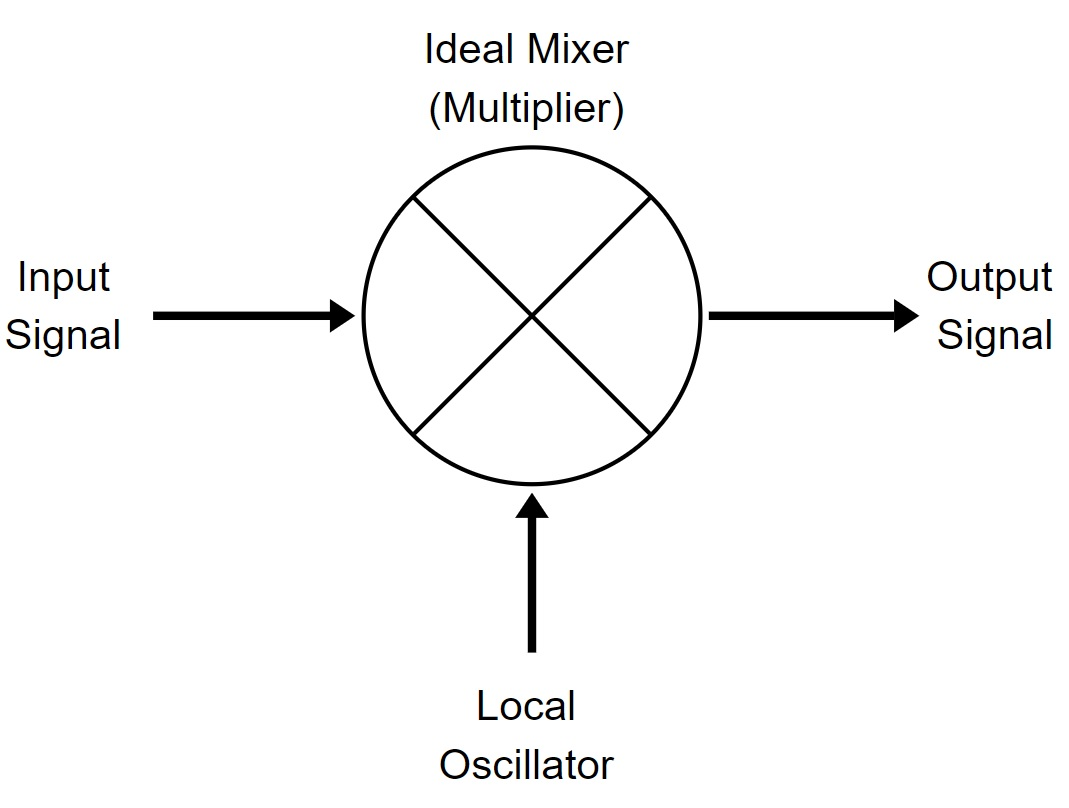
\includegraphics[scale=0.3]{imagenes/fig0.jpg}
	\caption{Mezclador ideal}\label{fig:fig0}
\end{figure}

En el proceso de recepción y transmisión de información en Radio Frecuencias son de fundamental utilidad los mezcladores. Cualquier dispositivo alineal puede ser un mezclador, diodos, transistores bipolares, FETs, etc. La no linealidad es necesaria para producir nuevas frecuencias. La elección del o dispositivo y del circuito depende de las consideraciones que se realicen sobre la ganancia o pérdida de conversión, rango dinámico, ancho de banda, figura de ruido, aislación entre los puertos, generación de frecuencias indeseables, costo y adaptación de sus puertos.

\begin{figure}[!ht]
  \centering    
	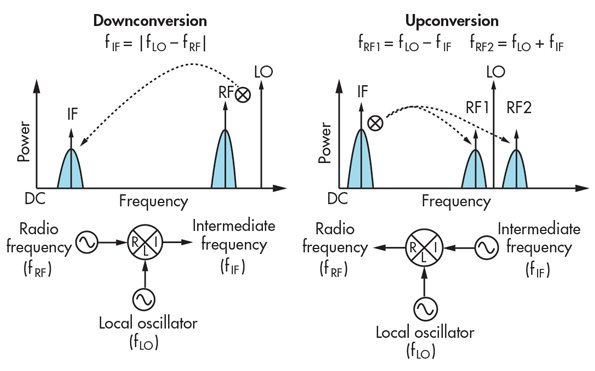
\includegraphics[scale=0.4]{imagenes/fig1.jpg}
	\caption{Esquema down-converter y up-converter}\label{fig:fig1}
\end{figure}

En cuanto a las características de la señal de salida, estos dispositivos pueden ser de dos tipos: uno se llama \textit{up}, donde la frecuencia de salida es mayor que la frecuencia de entrada y se emplean en procesos de transmisión; el otro tipo de mezclador se denomina \textit{down}, en este caso la frecuencia de salida es menor a la de entrada y se utiliza generalmente en procesos de recepción. Esto se representa en la figura \textcolor{blue}{\ref{fig:fig1}}

Como se mencionó anteriormente, en el proceso de recepción la señal de \textit{RF} es \textit{down converted}. El receptor cuenta con un oscilador local (LO) cuya frecuencia es determinada por la señal de \textit{RF} que se desea sintonizar. En la \textcolor{blue}{\ref{fig:fig2}} se muestra el espectro en frecuencia para un conversor de este tipo, donde $LO$ representa al oscilador local a la frecuencia $f_{LO}$ y \textit{RF} es la señal \textit{IF} a sintonizar a la frecuencia $f_{RF}$. La señal de \textit{RF} es mezclada con la señal del oscilador local produciendo la suma y diferencia de ambas frecuencias. La suma $f_{LO}$ $+$ $f_{RF}$ queda fuera de rango de operación del sistema y la diferencia $f_{LO}$ $-$ $f_{RF}$ es la señal de frecuencia intermedia \textit{IF} a la frecuencia $f_{IF}$, que es filtrada y amplificada. Es importante destacar que también aparece una señal imagen \textit{IM} a una frecuencia $f_{IM}$ que debe ser eliminada por el filtro de \textit{RF}. Dicho filtro debe ser suficientemente selectivo para eliminar esta componente imagen.

\begin{figure}[!ht]
  \centering    
	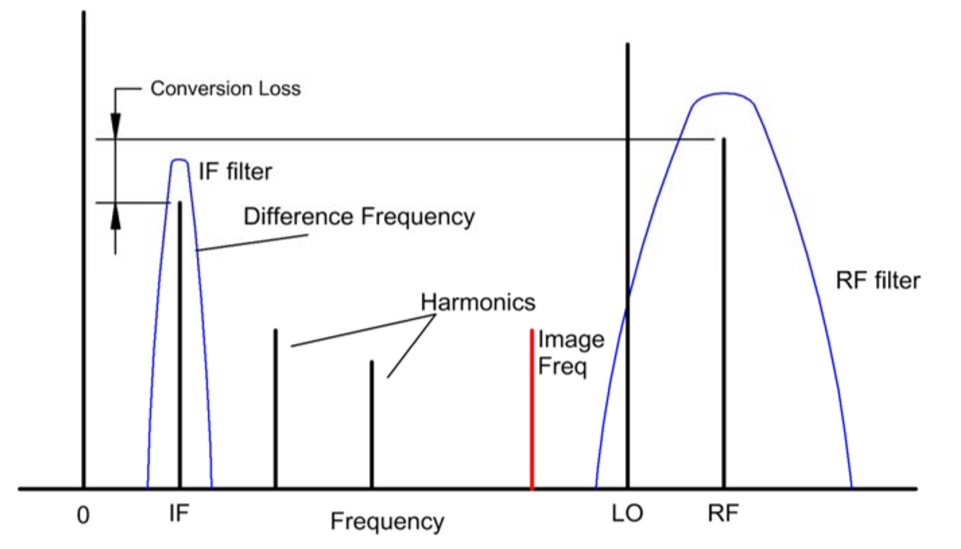
\includegraphics[scale=0.4]{imagenes/fig2.jpg}
	\caption{Frecuencias en un mezclador downconverter}\label{fig:fig2}
\end{figure}

Para el caso de un upconverter, la señal LO es multiplicada por la señal  resultando la \textit{RF} modulada en doble banda lateral con portadora suprimida. En otras palabras luego de realizar el producto se obtiene $f_{RF}$ = $f_{OL}$ $\pm$ $f_{IF}$, pero generalmente es usada solo una de estas señales de \textit{RF}, lo que hace necesaria también la implementación de un filtro.

Desde el punto de vista de la potencia, los mezcladores se clasifican en pasivos o activos. Un mezclador pasivo emplea diodos u otro dispositivo no lineal, donde la señal LO provee la potencia para producir la suma y la diferencia de frecuencias. Los mezcladores activos emplean FET o transistores alimentados con fuentes de tensión continua que proveen la potencia para el proceso de mezclado. 

\section{Definición de parámetros}
\subsection{Pérdida por conversión [CL]}
La Pérdida por Conversión ó \textit{Conversion Loss} para el caso particular de un conversor down, es definida como el cociente entre la señal de entrada \textit{RF} y la señal de salida \textit{IF} deseada.

\begin{figure}[!ht]
  \centering    
	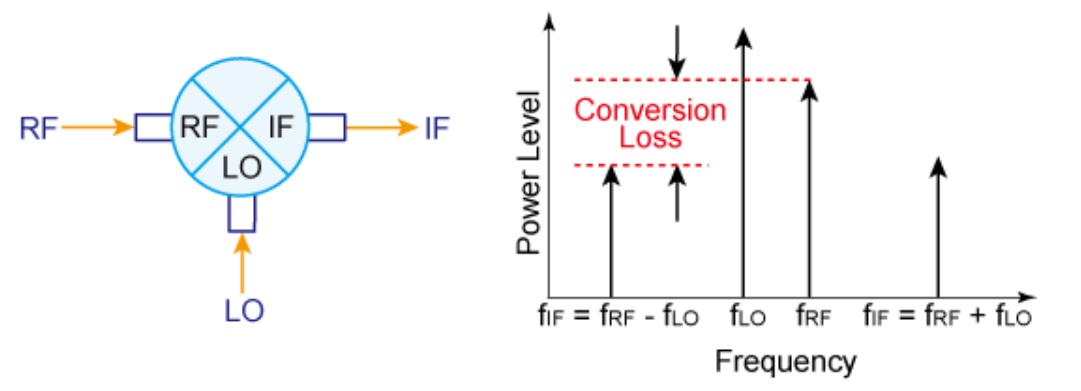
\includegraphics[scale=0.38]{imagenes/fig3.jpg}
	\caption{Perdida por conversión de un mezclador}\label{fig:fig3}
\end{figure}

Para el caso de un mezclador ideal, la potencia de entrada es divida a la mitad y distribuida en cada una de las dos componentes resultantes, produciendo un desplazamiento en frecuencia de la potencia. Entonces la pérdida por conversión se calcula como la relación entre la potencia de entrada y cualquiera de las resultantes de la mezcla:

\[CL = 10 \cdot log \left( \frac{P_{out} \; [mW]}{P_{in} [out]} \right) \]

\begin{equation}
CL = P_{in} \; [dBm]- P_{out} \; [dBm] \label{eq:1}
\end{equation}

En un mezclador pasivo ideal la perdida por conversión parte de $3 \; [dB]$ ya que se emplea solo una de las resultantes del producto. Para el caso de un mezclador práctico balanceado o doblemente balanceado este factor es menor a $6 \; [dB]$. La pérdida por conversión depende de la potencia aplicada por la señal del oscilador local y debe ser tenida en cuenta para el cálculo de la "Figura de Ruido". Es común, en receptores de calidad, el uso de un amplificador con ganancia mayor a este factor de pérdida para lograr que el mezclador afecte en menor medida la figura de ruido.

\subsection{Aislamiento [ISO]}
En la práctica se desea que exista una aislación entre los puertos \textit{LO}, \textit{RF} y \textit{IF} del mezclador, pero esto no siempre se cumple. La aislación entre un par de puertos A - B cuyas componentes fundamentales se encuentra en $f_A$ y $f_B$ respectivamente, se determina como la diferencia entre la potencia de la componente fundamental del puerto A y la potencia que posee la componente en la frecuencia $f_A$ del puerto B. En un mezclador de un solo diodo no suele existir aislamiento entre sus puertos. En el caso de los balanceados la aislación depende de las características de los diodos utilizados, por este motivo los fabricantes emplean dispositivos diseñados para tal fin. Un amplificador doble balanceado que hace uso de estos diodos particulares la aislación toma valores de $30 \; [dB]$. 

\subsection{Pérdidas por Compresión [CP]}
Para un mezclador down ideal la salida \textit{IF} debe ser proporcional a la señal de entrada \textit{RF}, en la práctica ocurre que a medida que la señal de entrada se aproxima a los $10\;[dB]$ por debajo de la potencia del oscilador local, la salida de frecuencia intermedia comienza a saturarse y la pérdida por conversión incrementa. Los fabricantes especifican el punto de $1 \; [dB]$ de compresión ya que se relaciona directamente con la potencia del oscilador local, un mayor valor de esta potencia permite lograr un punto de compresión de $1 \; [dB]$ más alto, incrementando el rango dinámico del mezclador. Se determina por medio de un barrido del parámetro $P_{RF}$ realizando una gráfica de la potencia de frecuencia intermedia $P_{IF}$ en función de $P_{RF}$. En un caso ideal, esta relación es lineal, sin embargo en la práctica para determinado valor de $P_{RF}$ esta relación se aleja de la linealidad. Definiendo entonces a la pérdida por compresión como el valor de $P_{RF}$ a partir del cual la gráfica real de $P_{IF}$ = $f(P_{RF})$ se aleja un decibel de la gráfica ideal. 

\begin{figure}[!ht]
  \centering    
	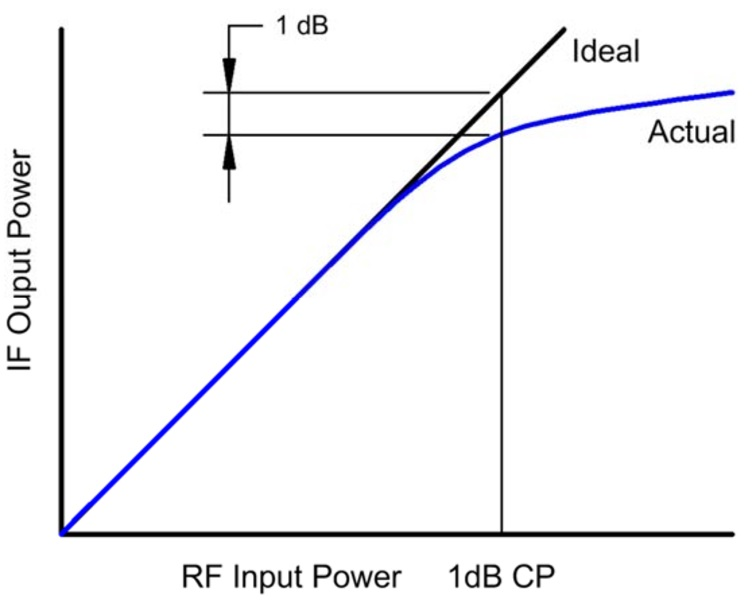
\includegraphics[scale=0.45]{imagenes/fig4.jpg}
	\caption{Punto de compresion de 1[dB] de un mezclador}\label{fig:fig4}
\end{figure}

\subsection{Figura de Ruido - Rango Dinámico}
 El rango dinámico se define como el grado de variación útil en que puede operar el mezclador. El valor superior del rango se encuentra determinado por el punto de compresión de $1 \; [dB]$ y el valor inferior es limitado por la figura de ruido. 

La figura de ruido es la cantidad de ruido aportado por el mixer a la señal convertida, sumada las pérdidas por conversión. Por definición, es el cociente entre la relación señal-ruido RF en la entrada y la relación señal-ruido FI en el puerto de salida, es decir, 
\begin{align*}
NF_{SSB} &= 10 \cdot log{\frac{SNR_i}{SNRo}} \\
		 &= 10 \cdot log{\frac{P_{RF_{in}}}{P_{N_{in}}}} - 10 \cdot \log{\frac{P_{IF_{out}}}{P_{N_{out}}}} \\
		 &= [P_{RF_{in}} - P_{IF_{out}}] + [P_{N_{out}} - P_{N_{in}}] \\
NF_{SSB} &= CL_{SSB} + P_{N_{mixer}}
\end{align*}

Se debe considerar que salvo solamente en casos específico de poseer diodos o transistores muy ruidosos, la figura de ruido es aproximadamente igual a la pérdida de conversión. En hojas de datos, generalmente, se especifica la figura de ruido de banda única ($NF_{SSB}$), ya que aunque el producto de la mezcla produce ambas bandas, inferior y superior, solo se desea uno de esos productos descartando el otro, causando que se pierda la mitad de la potencia de entrada y haciendo que la figura de ruido de banda lateral única esté 3 decibeles por encima de la figura de ruido de doble banda lateral ($NF_DSB$). Esta consideración se toma a menudo, debido a que medir la figura de ruido de doble banda lateral es sencillo.Se trata que sea lo menor posible para obtener un mayor rango dinámico de aplicación.

El ruido aportado, contiene principalmente 3 componentes: Térmico (Jhonson), ruido de disparo (Shot) y ruido de flicker. Generalmente, la figura de ruido de banda única está alrededor de los 0,5 dB por encima de la pérdida por conversión.

\subsection{Tipos de mezcladores}  
Según las exigencias del diseño, no en todos los casos se debe permitir que una o varias componentes de frecuencia aplicada en un puerto se filtren en otro, esto se define como la aislación entre puertos. Una forma de eliminar o atenúar estas componentes de frecuencia, es empleando un número par de dispositivos dispuestos en forma simétrica. Los tipos de mezcladores se pueden clasificar según su balanceo o equilibrio, es decir según la simetría de la configuración y paridad entre sus dispositivos. Las configuraciones más comunes son:

\begin{itemize}\itemsep0em
\item[•]  Mezcladores de terminación única.
\item[•]  Mezcladores de balanceo simple
\item[•]  Mezcladores de balanceo doble.
\end{itemize}

\clearpage

\section{Experiencia práctica}
Diseñar, calcular y simular diferentes mezcladores para ser utilizados en un receptor superheterodino de FM con las siguientes características:

\begin{itemize}\itemsep0em
\item[•]  $f_{IF} = 10,7 \; [Mhz]$.
\item[•]  $f_{RF} = 88-108 \; [Mhz]; \; P_{RF} = -10 \; [dBm]$.
\item[•]  $P_{LO} = 8 \;[dBm]$.
\end{itemize}

\subsection{Mezclador de terminación única}
Son aquellos mezcladores que emplean un único dispositivo alineal, ya sea un diodo o un transistor. Al poseer un solo dispositivo (impar), no hay simetrías que permitan eliminar frecuencias no deseadas en algunos de los terminales. En el caso de emplear un transistor, se logran niveles de aislación interesantes más por la unilateralidad que por simetría. Generalmente se emplean FETs, debido a su característica de transferencia más cuadrática que los BJT (generan menor cantidad de productos de intermodulación), permitiendo ganancias de conversión mayor que uno $(G_C = P_{IF}/P_{RF})$, y cierta aislación de \textit{OL} dada por la unilateralidad del dispositivo. En aplicaciones no muy comprometidas, su uso se justifica en los costos.

\subsubsection{Circuito}
La simulación se implementa en el software AWR. A continuación se muestra el esquemático
\begin{figure}[h]
  \centering    
	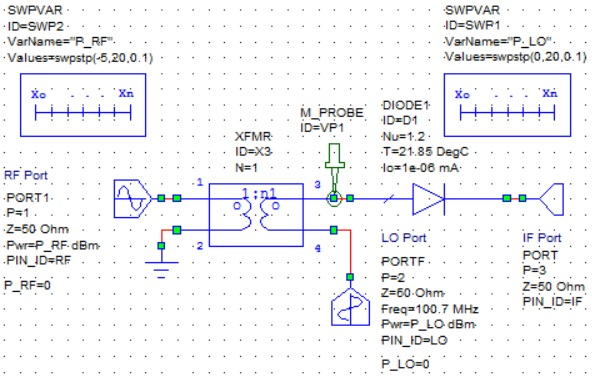
\includegraphics[scale=0.6]{imagenes/circuito1.jpg}
	\caption{Mezclador de terminación única con diodo.}\label{fig:circuito1}
\end{figure}

El circuito anterior produce el espectro de fourier de salida que se muestra en la figura \textcolor{blue}{\ref{fig:IF1}}.
\begin{figure}[h]
  \centering    
	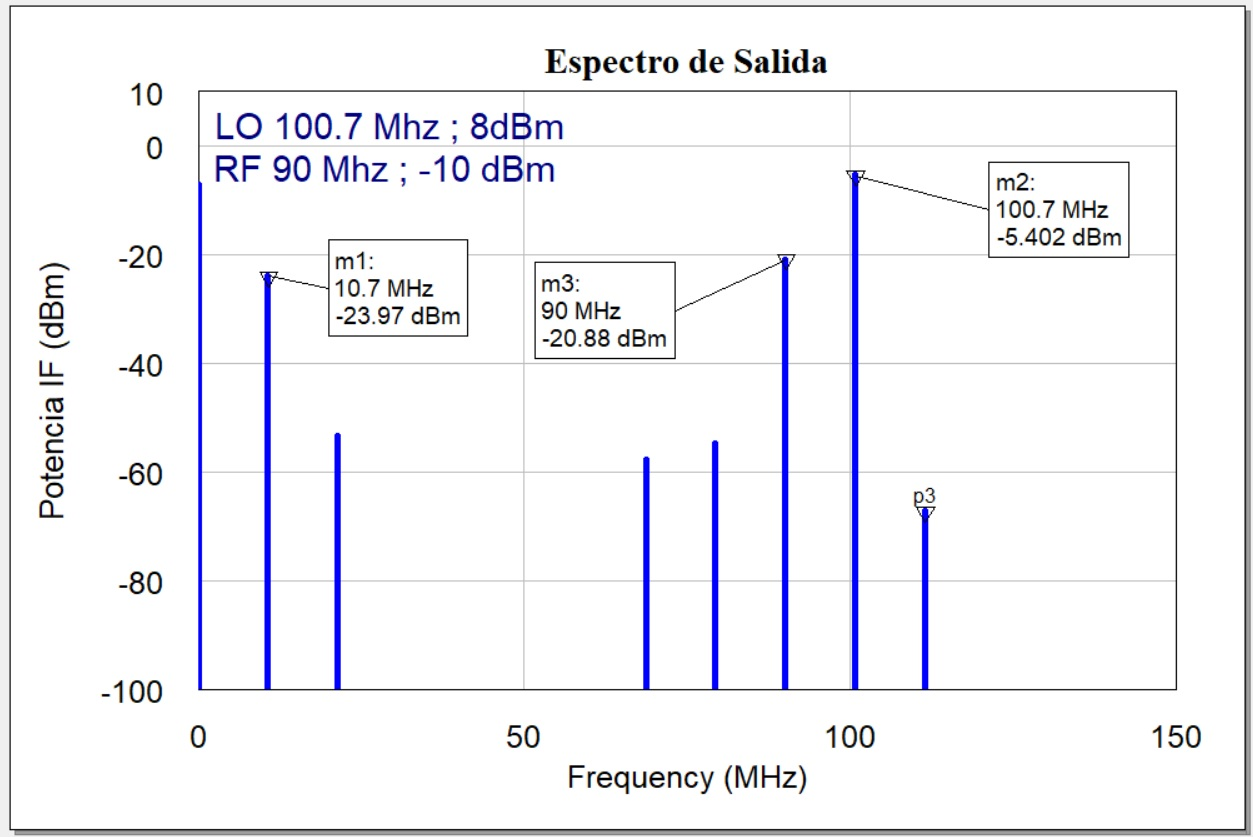
\includegraphics[scale=0.28]{imagenes/IF1.jpg}
	\caption{Espectro de Fourier de IF.}\label{fig:IF1}
\end{figure}
%
\subsubsection{Perdida por conversión}
%
\begin{figure}[h]
  \centering    
	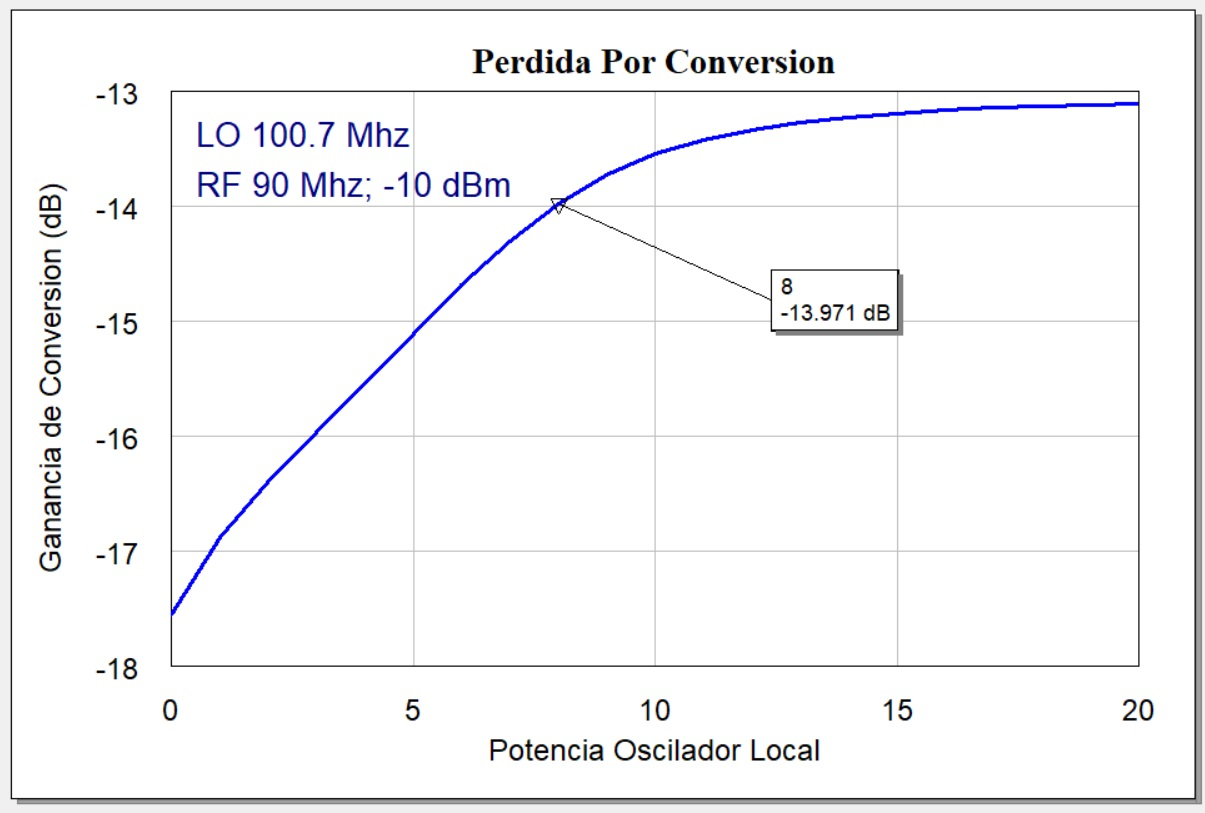
\includegraphics[width=\columnwidth]{imagenes/CL1.jpg}
	\caption{Perdida por conversión de mezclador terminación única.}\label{fig:CL1}
\end{figure}
\[C.L._{T.U.} = 13.971 \; [dB] \]
%
\subsubsection{Figura de ruido}
%
La figura de ruido se considera aproximadamente igual a la pérdida por conversión, excepto en los casos que se tengan diodos muy ruidosos.
\[N.F. \approx 13.971 \; [dB] \]
%
\subsubsection{Aislación entre puertos}
%
\begin{itemize}\itemsep0em
\item[•]  $ISO_{RF-IF} = 10,88 \; [dB]$.
\item[•]  $ISO_{LO-IF} = 13,40 \; [dB]$.
\item[•]  $ISO_{LO-RF} = 13,40 \; [dB]$.
\end{itemize}
%
\begin{figure}[h]
  \centering    
	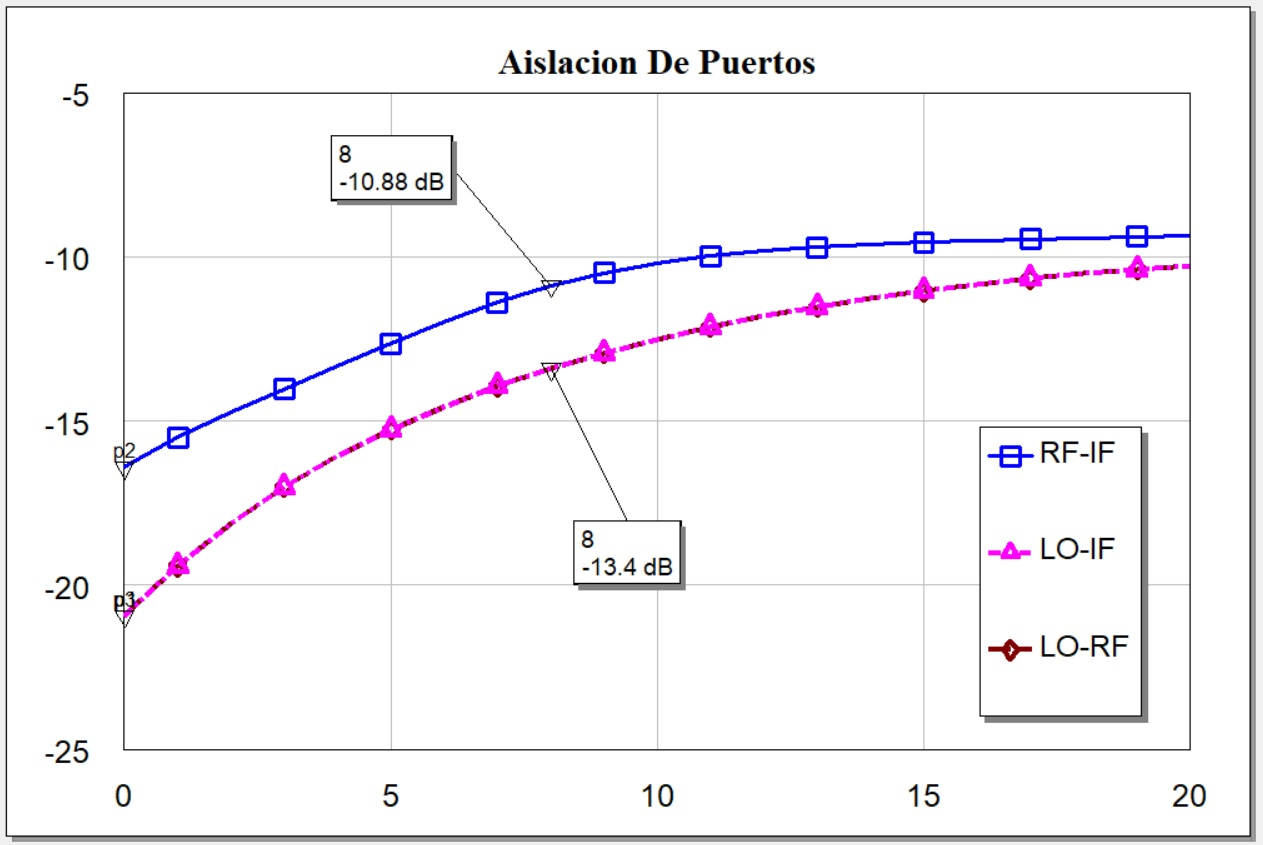
\includegraphics[width=\columnwidth]{imagenes/ISO1.jpg}
	\caption{Aislación entre puertos, terminación única.}\label{fig:ISO1}
\end{figure}
\clearpage
%
\subsubsection{Pérdida por compresión}
\begin{figure}[h!]
\centering
\begin{tikzpicture} [scale=1]
\begin{axis}[
	xmin=-5, xmax=20,
	ymin=-23.1, ymax=-12,
	xtick={-5,0,5.6,10,15,20},
	ytick={-14.9305,-13.886, -12, -16, -18, -20, -22},
    xlabel=Potencia del puerto RF,    
    ylabel=Potencia del puerto IF,
    legend pos=south east,
    grid=major,
    ]
    
	\addplot [red] 	table[x=LO,y=ideal] {tablas/CPL1.txt};  
	\addplot [blue] table[x=LO,y=RF] 	{tablas/CPL1.txt};
	\addplot[solid,
			mark=*, 
			mark options={solid,fill=yellow!80!black,draw=black, scale=0.5},
			black] 
			coordinates {(5.6,-13.886) (5.6,-14.9305)};

	\path [draw=gray, dashed, thick] (5.6,-14.9305) -- (5.6,-23);
	\path [draw=gray, dashed, thick] (5.6,-14.9305) -- (-6,-14.9305);
	\path [draw=gray, dashed, thick] (5.6,-13.886)  -- (-6,-13.886);
	
	\draw [decorate, decoration={brace,amplitude=2pt,raise=1pt}] (5.6,-13.886)  -- (5.6,-14.9305) node [midway, anchor=south west,yshift=-1mm, outer sep=1pt,font=\tiny]{1dB};
	
	\addlegendentry{Ideal}
	\addlegendentry{Real}
\end{axis}
\end{tikzpicture}
	\caption{Perdida por compresión terminación única}
\end{figure}

Perdida por compresión = $5.6 \; [dB]$

\subsection{Mezcladores de balanceo simple}
Este tipo de mezclador posee un par de dispositivos alineales, normalmente diodos o FETs, dispuestos en forma equilibrada de tal manera que el terminal de entrada quede aislado de los otros dos terminales.

\subsubsection{Circuito}
La simulación se implementa en el software AWR. A continuación se muestra el esquemático
\begin{figure}[h]
  \centering    
	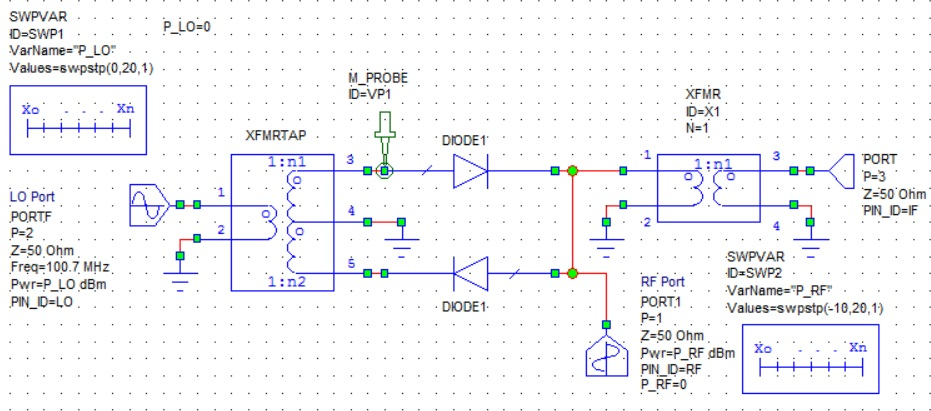
\includegraphics[width=\columnwidth]{imagenes/circuito2.jpg}
	\caption{Mezclador de balanceo simple.}\label{fig:circuito2}
\end{figure}

El circuito anterior produce el espectro de Fourier de salida que se muestra en la figura \textcolor{blue}{\ref{fig:IF2}}.
\begin{figure}[h]
  \centering    
	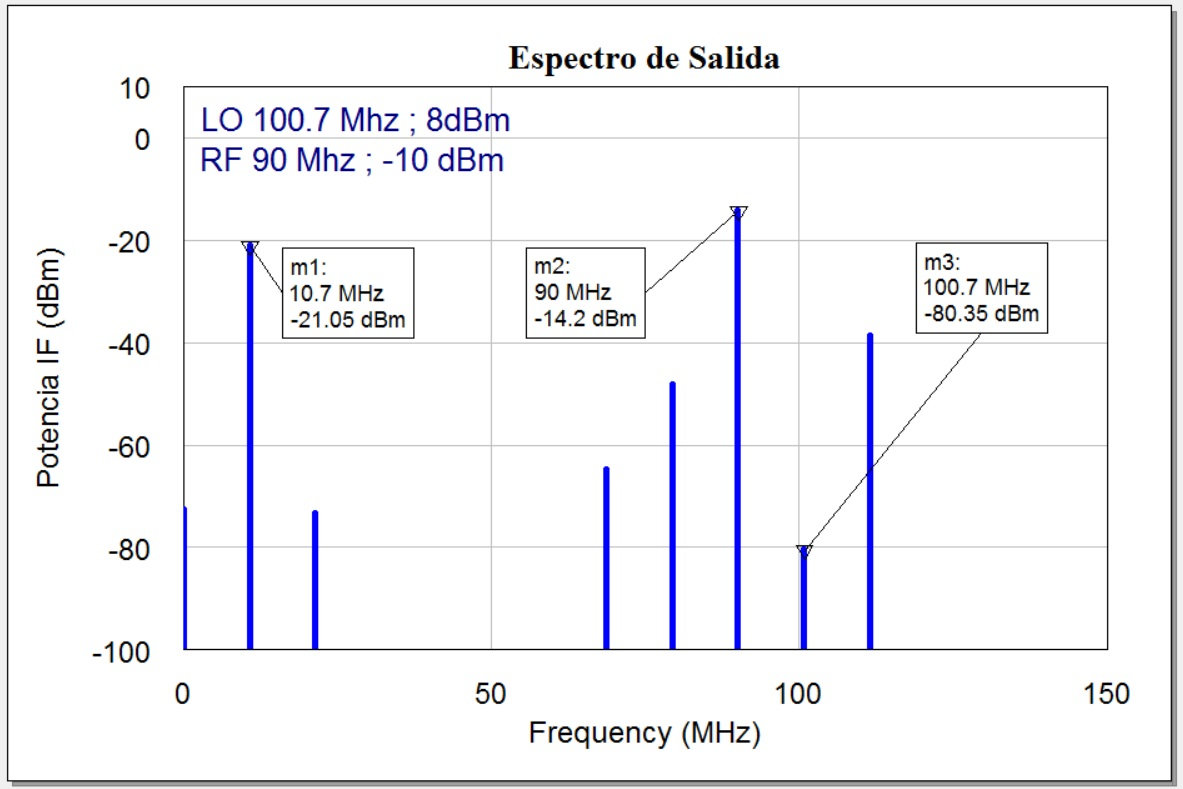
\includegraphics[width=\columnwidth]{imagenes/IF2.jpg}
	\caption{Espectro de Fourier de IF.}\label{fig:IF2}
\end{figure}
%
\subsubsection{Perdida por conversión}
%
\begin{figure}[h]
  \centering    
	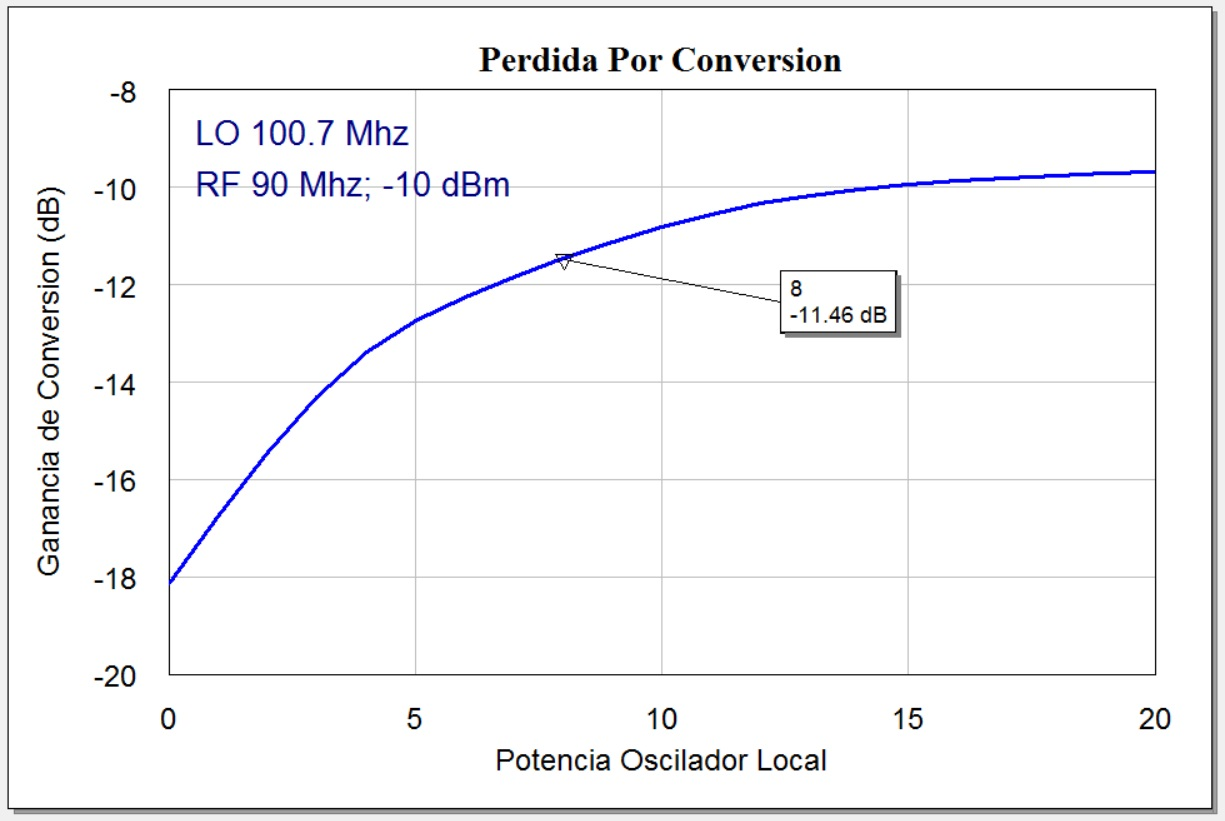
\includegraphics[width=\columnwidth]{imagenes/CL2.jpg}
	\caption{Perdida por conversión de mezclador de balanceo simple.}\label{fig:CL2}
\end{figure}
\[C.L._{B.S.} = 11.46 \; [dB] \]
%
\subsubsection{Figura de ruido}
%
La figura de ruido se considera aproximadamente igual a la pérdida por conversión, excepto en los casos que se tengan diodos muy ruidosos.
\[N.F. \approx 11.46 \; [dB] \]
%
\subsubsection{Aislación entre puertos}
%
\begin{itemize}\itemsep0em
\item[•]  $ISO_{RF-IF} = 4,204 \; [dB]$.
\item[•]  $ISO_{LO-IF} = 88,35 \; [dB]$.
\item[•]  $ISO_{LO-RF} = 88,35 \; [dB]$.
\end{itemize}
%
\begin{figure}[h!]
  \centering    
	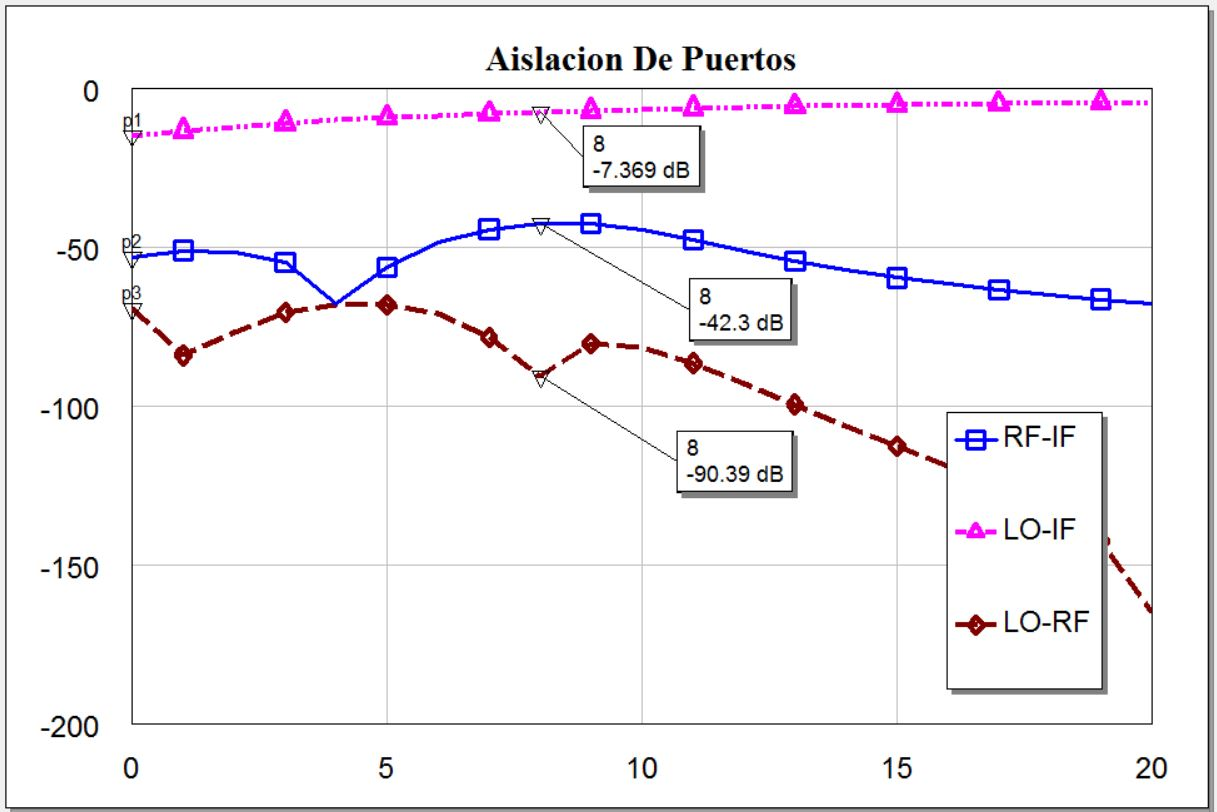
\includegraphics[scale=0.3]{imagenes/ISO2.jpg}
	\caption{Aislación entre puertos, balanceo simple.}\label{fig:ISO2}
\end{figure}
\clearpage
%
\subsubsection{Pérdida por compresión}
\begin{figure}[h!]
\centering
\begin{tikzpicture} [scale=1]
\begin{axis}[
	xmin=0, xmax=20,
	ymin=-18, ymax=-5,
	xtick={0,5,10,11.5,15,20},
	ytick={-6, -9.02058,-8,-10 , -12, -14, -16, -18},
    xlabel=Potencia del puerto RF,    
    ylabel=Potencia del puerto IF,
    legend pos=south east,
    grid=major,
    ]
    
	\addplot [red] 	table[x=LO,y=ideal] {tablas/CPL4.txt};  
	\addplot [blue] table[x=LO,y=RF] 	{tablas/CPL4.txt};
	\addplot[solid,
			mark=*, 
			mark options={solid,fill=yellow!80!black,draw=black, scale=0.5},
			black] 
			coordinates {(11.5,-8) (11.5,-9.02058)};

	\path [draw=gray, dashed, thick] (11.5,-9.02058) -- (11.5,-23);
	\path [draw=gray, dashed, thick] (11.5,-9.02058) -- (-6,-9.02058);
	\path [draw=gray, dashed, thick] (11.5,-8)  -- (-6,-8);
	
	\draw [decorate, decoration={brace,amplitude=2pt,raise=1pt}] (11.5,-8)  -- (11.5,-9.02058) node [midway, anchor=south west,yshift=-1mm, outer sep=1pt,font=\tiny]{1dB};
	
	\addlegendentry{Ideal}
	\addlegendentry{Real}
\end{axis}
\end{tikzpicture}
	\caption{Perdida por compresión de mezclador de balanceo simple}
\end{figure}
%
Perdida por compresión = $11,5 \; [dB]$
%
\subsection{Mezcladores de balanceo doble}
Todos los terminales están aislados entre sí, por lo que las frecuencias de las señales de entrada no aparecen a la salida. Los dos transformadores proveen aislación a todos los puertos, de esta forma se evita que las componentes de LO aparezcan en otros puertos o mejor dicho se vea reducida. Es necesario que la implementación de este puente sea equilibrado para así obtener un perfecto bloqueo de la señal.

\subsubsection{Circuito}
La simulación se implementa en el software AWR. A continuación se muestra el esquemático
\begin{figure}[h]
  \centering    
	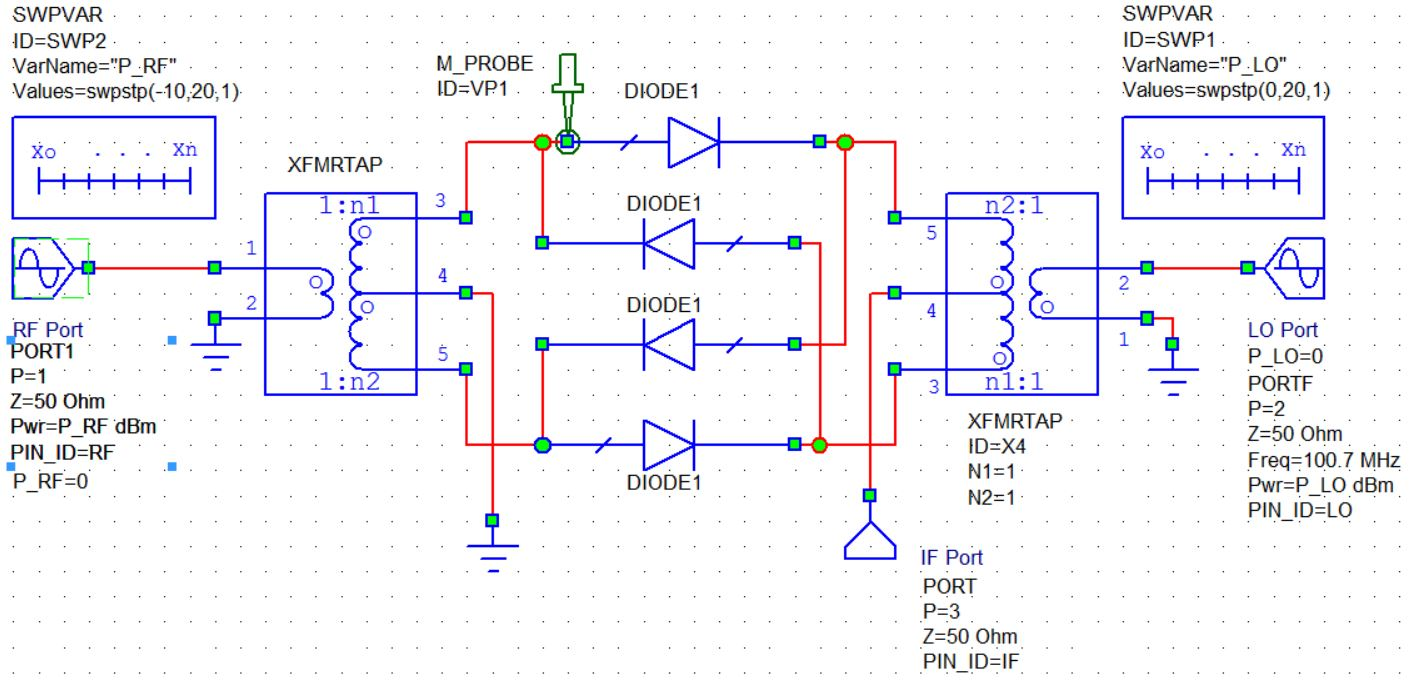
\includegraphics[width=\columnwidth]{imagenes/circuito3.jpg}
	\caption{Mezclador de balanceo doble.}\label{fig:circuito3}
\end{figure}

El circuito anterior produce el espectro de Fourier de salida que se muestra en la figura \textcolor{blue}{\ref{fig:IF3}}.
\begin{figure}[h]
  \centering    
	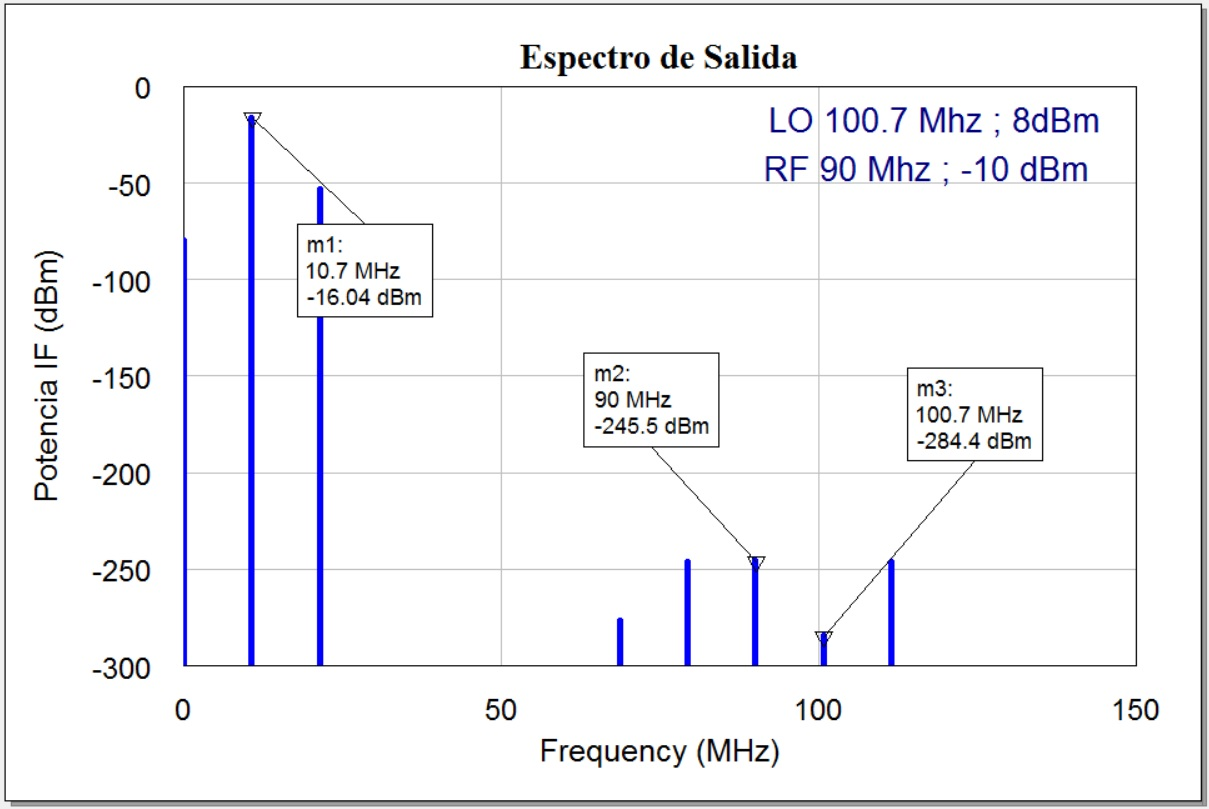
\includegraphics[scale=0.3]{imagenes/IF3.jpg}
	\caption{Espectro de Fourier de IF.}\label{fig:IF3}
\end{figure}
%
\subsubsection{Perdida por conversión}
%
\begin{figure}[h]
  \centering    
	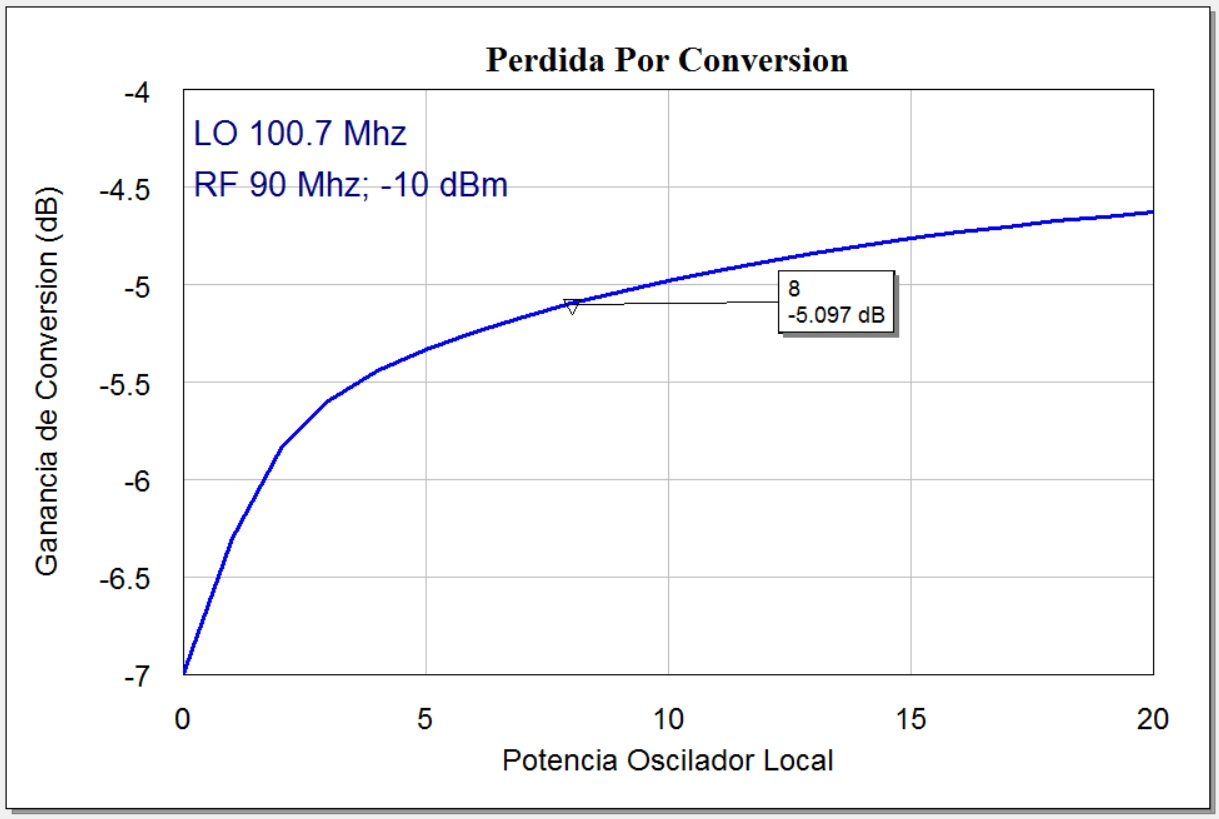
\includegraphics[scale=0.3]{imagenes/CL3.jpg}
	\caption{Perdida por conversión de mezclador de balanceo doble.}\label{fig:CL3}
\end{figure}
\[C.L._{B.D.} = 5.097 6 \; [dB] \]
%
\subsubsection{Figura de ruido}
%
La figura de ruido se considera aproximadamente igual a la pérdida por conversión, excepto en los casos que se tengan diodos muy ruidosos.
\[N.F. \approx 5.097 \; [dB] \]
%
\subsubsection{Aislación entre puertos}
%
\begin{itemize}\itemsep0em
\item[•]  $ISO_{RF-IF} = 235,5 \; [dB]$.
\item[•]  $ISO_{LO-IF} = 292,4 \; [dB]$.
\item[•]  $ISO_{LO-RF} = 92.02 \; [dB]$.
\end{itemize}
%
\begin{figure}[h]
  \centering    
	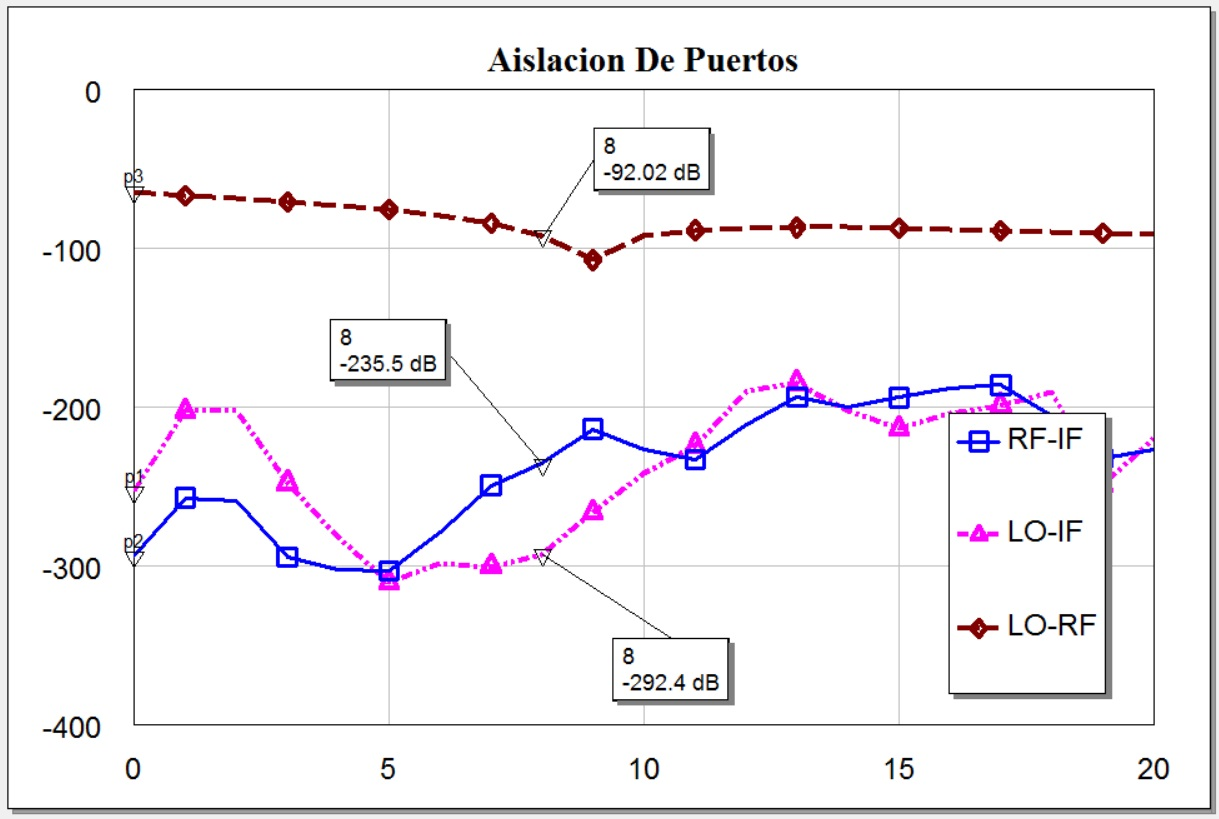
\includegraphics[scale=0.3]{imagenes/ISO3.jpg}
	\caption{Aislación entre puertos, balanceo doble.}\label{fig:ISO3}
\end{figure}
\clearpage
%
\subsubsection{Pérdida por compresión}
\begin{figure}[h!]
\centering
\begin{tikzpicture} [scale=1]
\begin{axis}[
	xmin=-5, xmax=20,
	ymin=-12, ymax=-3,
	xtick={0,2.6,5,10,15,20, -5},
	ytick={-4.44354,-5.48021, -10, -8, -12, -6, -4},
    xlabel=Potencia del puerto RF,    
    ylabel=Potencia del Puerto IF,
    legend pos=south east,
    grid=major,
    ]
    
	\addplot [red] 	table[x=LO,y=ideal] {tablas/CPL3.txt};  
	\addplot [blue] table[x=LO,y=RF] 	{tablas/CPL3.txt};
	\addplot[solid,
			mark=*, 
			mark options={solid,fill=yellow!80!black,draw=black, scale=0.5},
			black] 
			coordinates {(2.6,-5.48021) (2.6,-4.44354)};

	\path [draw=gray, dashed, thick] (2.6,-4.44354) -- (2.6,-23);
	\path [draw=gray, dashed, thick] (2.6,-4.44354) -- (-6,-4.44354);
	\path [draw=gray, dashed, thick] (2.6,-5.48021)  -- (-6,-5.48021);
	
	\draw [decorate, decoration={brace,amplitude=6pt,raise=1pt}] (2.6,-5.48021)  -- (2.6,-4.44354) node [midway, anchor=south east,yshift=-3.5mm, outer sep=6pt,font=\tiny]{1dB};
	
	\addlegendentry{Ideal}
	\addlegendentry{Real}
\end{axis}
\end{tikzpicture}
	\caption{Pérdida por compresión de mezclador de balanceo doble.
	}
\end{figure}

Perdida por compresión = $2.6\; [dB]$

\section{Conclusión}
 Como modo de finalizar se agrupan los valores obtenidos en las siguientes tablas
\begin{table}[h]
	\centering
  \begin{threeparttable}
     \begin{tabular}{lccc}
        \toprule
        Mixer 				& $C.L.$ 	& $C.P.$ 	& $N.F.$  \\
        \midrule
        Terminacion Unica   & 13,971   	& 5,6    	& 13,971 \\
        Balanceo Simple     & 11,46   	& 11,5    	& 11,46	 \\
        Balanceo Doble    	& 5,097     & 2,6    	& 5,097  \\
        \bottomrule
     \end{tabular}
    \begin{tablenotes}
      \small
      \item Valores en dB.
    \end{tablenotes}
    \caption{Perdida por conversión, compresión y figura de ruido.}
  \end{threeparttable}
\end{table}

\begin{table}[h]
	\begin{adjustbox}{width=\columnwidth,center}
  \begin{threeparttable}
     \begin{tabular}{lccc}
        \toprule
        Mixer 				&$ISO_{(RF-IF)}$ 	& $ISO_{(LO-IF)}$ 	& $ISO_{(LO-RF)}$ \\
        \midrule
        Terminacion Unica   & 10,88        		& 13,40    			& 13,40 \\
        Balanceo Simple     & 4,204        		& 88,35    			& 88,35 \\
        Balanceo Doble    	& 235,5        		& 292,4    			& 92,02 \\
        \bottomrule
     \end{tabular}
    \begin{tablenotes}
      \small
      \item Valores en dB.
    \end{tablenotes}
    \caption{Aislaciones entre puertos}
  \end{threeparttable}
  \end{adjustbox}
\end{table}

Observando los resultados obtenidos se estableció una comparación entre los 3 tipos de configuraciones analizadas, considerando que se independizó del dispositivo alineal empleado, ya que se empleó un diodo genérico para los 3 casos, y que existen programas de simulación que imitan en mayor medida el comportamiento y las condiciones reales en RF. 

Analizando desde el punto de vista de la aislación entre puertos, el esquema de doble balance posee un mejor desempeño, ya que existe una aislación total (galvánica) en ambos sentidos, entre los 3 puertos, producto del empleo de transformadores de punto medio donde los amperes por vuelta de cada secundario son iguales y están en contrafase, anulando cualquier componente de cada puerto en los demás, lo que se visualiza en los espectros de la simulación. Esto hace notar la relevancia de la paridad entre los dispositivos alineales. Luego, en el circuito de balance simple se observa una aislación total, en este caso, solamente en el puerto del oscilador, mientras que los demás puertos poseen una aislación nula y que se podría compensar mediante el uso de filtros. Por último, en la configuración de terminación única se puede remarcar que existe algún tipo de aislación desde el puerto FI hacia los demás puertos, debido a la unilateralidad del diodo.

Por otro lado, analizando las pérdidas por conversión se visualiza que el mezclador de doble posee el mejor rendimiento, convirtiendo en mayor medida la potencia de entrada RF en potencia de salida FI. 

Observando las figuras de ruido de banda única, no se puede establecer un criterio de comparación debido a que el ruido aportado por los dispositivos es despreciable, simplificando el criterio a que la figura de ruido sea idéntica a las pérdidas por conversión. 

 Una configuración de terminación única se lo emplea en aplicaciones donde se busca reducir costes o donde existen frecuencias muy elevadas, destacando su simplicidad y añadiendo solamente filtros selectivos.
 
 Si bien todas las características del la configuración de balance doble son buenas, hay que poner en el otro extremo de la balanza la complejidad, costo y volumen que significa en comparación con las otras topologías analizadas.


\end{document}